\section*{Autores}

\begin{wrapfigure}{l}{0.3\linewidth}
\includegraphics[width=\linewidth]{}  
\end{wrapfigure}

\textbf{Igor Galvão de Melo} é graduando em Engenharia de Computação pelo Instituto Nacional de Telecomunicações - Inatel. Estagiário na área de engenharia de vendas, e possui interesses na área de programação, vendas, planejamento e gerenciamento.

\begin{wrapfigure}{l}{0.3\linewidth}
\end{wrapfigure}

   \textbf{Lucas José Silva Corrêa} é graduando em Engenharia de Computação pelo Inatel - Instituto Nacional de Telecomunicações. Estagiário na área de soft no Inatel Competence Center - ICC. Possui interesse nas áreas de Tecnologia, DevOps e programação.\newline

\begin{wrapfigure}{l}{0.3\linewidth}
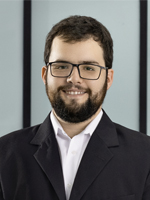
\includegraphics[width=\linewidth]{figuras/autor5.jpg}  
\end{wrapfigure}

    \textbf{Marcelo Vinícius Cysneiros Aragão} é graduado em Engenharia de Computação pelo Instituto Nacional de Telecomunicações (Inatel) em 2014 e Mestre em Ciência e Tecnologia da Computação pela Universidade Federal de Itajubá em 2018. Trabalhou de 2011 a 2018 no Inatel Competence Center, mais recentemente como Especialista em Sistemas, onde atuou principalmente como desenvolvedor de soluções de Business Support Systems (BSS) em ambiente de integração contínua. É professor de disciplinas da graduação, como Engenharia de Software e Redes Neurais, e coordenador do curso de pós-graduação em Desenvolvimento de Aplicações para Dispositivos Móveis e Cloud Computing. Possui interesse nas áreas de análise de algoritmos, desenvolvimento de software, inteligência artificial, aprendizado de máquina e ciência de dados.